\documentclass[tikz, convert = false]{standalone}%

\usepackage[utf8]{inputenx}%  http://ctan.org/pkg/inputenx
% Euler for math | Palatino for rm | Helvetica for ss | Courier for tt
\renewcommand{\rmdefault}{ppl}% rm
\linespread{1.05}% Palatino needs more leading
\usepackage[scaled]{helvet}% ss //  http://ctan.org/pkg/helvet
\usepackage{courier}% tt // http://ctan.org/pkg/courier
\usepackage{eulervm}  %  http://ctan.org/pkg/eulervm
% a better implementation of the euler package (not in gwTeX)
\normalfont%
\usepackage[T1]{fontenc}%  http://ctan.org/pkg/fontenc
\usepackage{textcomp}%  http://ctan.org/pkg/textcomp

\usepackage{fp}
\usetikzlibrary{calc}
\usetikzlibrary{intersections}
\usetikzlibrary{fixedpointarithmetic}

\begin{document}
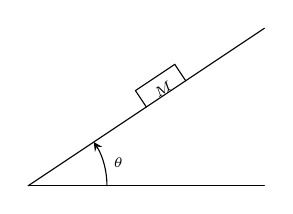
\begin{tikzpicture}[line join = round, line cap = round]
  \coordinate (O) at (0, 0);

  \draw (O) -- +(3, 0) coordinate (P1);
  \draw[name path = sline] (O) -- (3, 2) coordinate (P2);

  \draw[-stealth] let
    \p0 = (O),
    \p1 = (P1),
    \p2 = (P2),
    \n1 = {atan2(\y1 - \y0, \x1 - \x0)},
    \n2 = {atan2(\y2 - \y0, \x2 - \x0)},
    \n3 = {1cm},
    \n4 = {(\n1 + \n2)/2}
  in \pgfextra{\xdef\myn{\n2}} (O) +(\n1:\n3) arc[radius = \n3,
  start angle = \n1, end angle = \n2] node[right, font = \tiny] at (\n4:\n3)
  {$\theta$};

  \path[name path = line1] (1.5, 0) -- +(0, 1.25);
  \path[name path = line2] (2, 0) -- +(0, 1.5);
  \path[name intersections = {of = sline and line1, by = P3}];
  \path[name intersections = {of = sline and line2, by = P4}];
  
  \draw (P3) -- ($(P3)!.25cm!-90:(O)$) coordinate (P5);
  \draw (P4) -- ($(P4)!.25cm!-90:(O)$) coordinate (P6);
  \draw (P5) -- (P6) node[pos = .5, below, font = \tiny, rotate = \myn] {$M$};
\end{tikzpicture}
\end{document}
%%% Local Variables:
%%% mode: latex
%%% TeX-master: t
%%% End:
